\documentclass[11pt,a4paper]{article}

% ------------------------------------------------------------------
% Packages
% ------------------------------------------------------------------
\usepackage[margin=2.5cm]{geometry}
\usepackage[T1]{fontenc}
\usepackage{lmodern}
\usepackage{graphicx}
\usepackage{subcaption}
\usepackage{booktabs}
\usepackage{amsmath}
\usepackage{float}
\usepackage{xcolor}
\usepackage[hidelinks]{hyperref}
\usepackage{siunitx}
\sisetup{group-separator={,}, group-minimum-digits=4}

% Figures are read from the project's figures/ folder.
\graphicspath{{../figures/}}

\title{\textbf{Food Customers: Exploratory Data Analysis}\\[0.3em]
\large MAS531 Group Project ``Fo''}
\author{Davide \and Fanourios Loucas \and Olga \and Panagiotis}
\date{November 2026}

\begin{document}
\maketitle

\begin{abstract}
We analyse the marketing data of a food company (2,205 customers, 27 variables) to describe its customers and the relationships between their characteristics and their purchasing behaviour. After removing 203 duplicate rows and 5 inconsistent records, 1,997 customers remain. None of the numerical variables is normally distributed, so non-parametric methods are used throughout. Income is by far the strongest driver of spending (Spearman $\rho = 0.87$). Customers with children spend much less (median 182 vs 1,117) and rely far more on discounts, and this effect remains at the same income level. Education and marital status have little or no effect once income is taken into account. A k-means clustering identifies three customer segments: \emph{budget families}, \emph{affluent big spenders} and \emph{established families}.
\end{abstract}

\tableofcontents
\newpage

% ==================================================================
\section{Introduction}
% ==================================================================
The company wants a full exploratory analysis of its customer data in order to understand the profiles of its customers and how the variables vary together. Our aims are to:
\begin{enumerate}
  \item clean the data and check it for errors and inconsistencies;
  \item describe each variable (summary statistics, plots, distribution shape);
  \item study the relationships between variables, especially with total spending;
  \item test the most important patterns formally with hypothesis tests;
  \item group customers into segments and measure the effect of each characteristic on spending.
\end{enumerate}
All analysis was done in R. The code is submitted with this report and is commented section by section.

% ==================================================================
\section{Data}
% ==================================================================
The dataset contains 2,205 customers and 27 variables:
\begin{itemize}
  \item \textbf{Profile:} \texttt{Income} (annual household income), \texttt{Age}, \texttt{Kidhome} (small children at home), \texttt{Teenhome} (teenagers at home), marital status (5 indicator columns) and education (4 indicator columns).
  \item \textbf{Spending in the last 2 years:} on wine, fruit, meat, fish and sweet products (\texttt{Mnt*}), and the total, \texttt{Total\_amount\_spent}.
  \item \textbf{Purchases:} number of purchases through the website, the catalogue and in stores, the number made with a discount, and website visits in the last month.
  \item \textbf{Relationship with the company:} \texttt{Customer\_Days} (days as a customer), \texttt{Recency} (days since the last purchase) and \texttt{Complain} (complained in the last 2 years).
\end{itemize}

% ==================================================================
\section{Data Cleaning and Preparation}
% ==================================================================

\subsection{Missing values and duplicates}
There are no missing values. However, 203 rows are identical to another row in all 27 columns, including the exact income and the exact number of days as a customer. Two different customers matching on every column is very unlikely, so these rows were treated as repeated entries and removed (2,205 $\to$ 2,002 customers).

\subsection{Logic checks}
We ran 13 checks to make sure the values are consistent with each other (Table~\ref{tab:checks}). Three of them failed for a few customers:
\begin{itemize}
  \item 4 customers made 0 purchases but spent 4--8, which is impossible. They were removed.
  \item 1 customer made more discount purchases than purchases in total. This customer was removed.
\end{itemize}
After cleaning, \textbf{1,997 customers} remain. Check 1 also shows that \texttt{Total\_amount\_spent} is exactly the sum of the five \texttt{Mnt*} columns, so it is never used in the same test or model as those columns. Check 13 found 4 customers who were 16--18 years old when they joined. This is possible, so they were kept.

\begin{table}[H]
\centering
\small
\begin{tabular}{rlc}
\toprule
\# & Check & Result \\
\midrule
1 & Total spent equals the sum of the \texttt{Mnt*} columns & Pass \\
2 & No customer with 0 purchases has spent money & 4 removed \\
3 & Discount purchases do not exceed total purchases & 1 removed \\
4 & Each customer has exactly one marital status & Pass \\
5 & Each customer has exactly one education level & Pass \\
6 & Indicator columns contain only 0 or 1 & Pass \\
7 & No negative values & Pass \\
8 & All counts and amounts are whole numbers & Pass \\
9 & \texttt{Kidhome} and \texttt{Teenhome} only take values 0--2 & Pass \\
10 & Income is positive and age is realistic (24--80) & Pass \\
11 & Last purchase is not before the customer joined & Pass \\
12 & No customer with purchases has spent nothing & Pass \\
13 & Age when joining (4 customers were 16--18) & Kept \\
\bottomrule
\end{tabular}
\caption{Logic checks on the data.}
\label{tab:checks}
\end{table}

\subsection{New variables}
The indicator columns were combined into two categorical variables, as suggested in the project description:
\begin{itemize}
  \item \texttt{Marital\_State}: Divorced, Living together, Married, Single or Widow.
  \item \texttt{schoolinglevel}: an ordered factor, high school $<$ bachelor's $<$ master's $<$ PhD.
\end{itemize}
We also created:
\begin{itemize}
  \item \texttt{Children} = \texttt{Kidhome} + \texttt{Teenhome} (0--3), and \texttt{HasChildren} (yes/no);
  \item \texttt{TotalPurchases} = web + catalogue + store purchases;
  \item \texttt{AgeGroup}: under 30, 30--44, 45--59, 60+;
  \item \texttt{IncomeGroup}: income quartiles (boundaries \num{35641}, \num{51529} and \num{68352});
  \item \texttt{WebPercent}, \texttt{CataloguePercent}, \texttt{StorePercent}: the share of each customer's purchases made through each channel (\%);
  \item \texttt{DealPercent}: the share of each customer's purchases made with a discount (\%).
\end{itemize}

% ==================================================================
\section{Univariate Analysis}
% ==================================================================

\subsection{Numerical variables}
Table~\ref{tab:desc} summarises the 15 numerical variables. All values are in a sensible range.

\begin{table}[H]
\centering
\small
\begin{tabular}{l S[table-format=4.0] S[table-format=5.0] S[table-format=5.1] S[table-format=5.1] S[table-format=6.0] S[table-format=-1.2]}
\toprule
Variable & {Min} & {Median} & {Mean} & {SD} & {Max} & {Skewness} \\
\midrule
Income              & 2447 & 51529 & 51803.5 & 20618.9 & 113734 & 0.01 \\
Age                 & 24   & 50    & 51.2    & 11.7    & 80     & 0.09 \\
Recency             & 0    & 49    & 49.0    & 29.0    & 99     & -0.01 \\
Customer\_Days      & 2159 & 2510  & 2511.3  & 202.0   & 2858   & 0.00 \\
MntWines            & 0    & 179   & 306.6   & 337.0   & 1493   & 1.16 \\
MntFruits           & 0    & 8     & 26.5    & 39.9    & 199    & 2.09 \\
MntMeatProducts     & 0    & 69    & 166.5   & 219.5   & 1725   & 1.82 \\
MntFishProducts     & 0    & 12    & 37.8    & 55.0    & 259    & 1.91 \\
MntSweetProducts    & 0    & 8     & 27.4    & 41.6    & 262    & 2.10 \\
Total\_amount\_spent& 6    & 345   & 564.9   & 576.1   & 2491   & 0.91 \\
NumDealsPurchases   & 0    & 2     & 2.3     & 1.8     & 15     & 2.13 \\
NumWebPurchases     & 0    & 4     & 4.1     & 2.8     & 27     & 1.24 \\
NumCatalogPurchases & 0    & 2     & 2.7     & 2.8     & 28     & 1.40 \\
NumStorePurchases   & 0    & 5     & 5.8     & 3.2     & 13     & 0.72 \\
NumWebVisitsMonth   & 0    & 6     & 5.3     & 2.4     & 20     & -0.01 \\
\bottomrule
\end{tabular}
\caption{Summary statistics of the numerical variables (1,997 customers).}
\label{tab:desc}
\end{table}

The main observations are:
\begin{itemize}
  \item \textbf{Spending is strongly right-skewed.} For every \texttt{Mnt*} column the mean is far above the median (e.g.\ fruit: median 8, mean 26.5). Most customers spend little, and a few spend a lot (Figure~\ref{fig:uni}).
  \item \textbf{Purchase counts are also right-skewed}, especially discount, web and catalogue purchases.
  \item \textbf{Recency and Customer\_Days are roughly flat (uniform)}: customers are spread evenly over the range.
  \item \textbf{Income and Age are roughly symmetric} with one main peak.
\end{itemize}

\begin{figure}[H]
\centering
\begin{subfigure}{0.48\textwidth}
  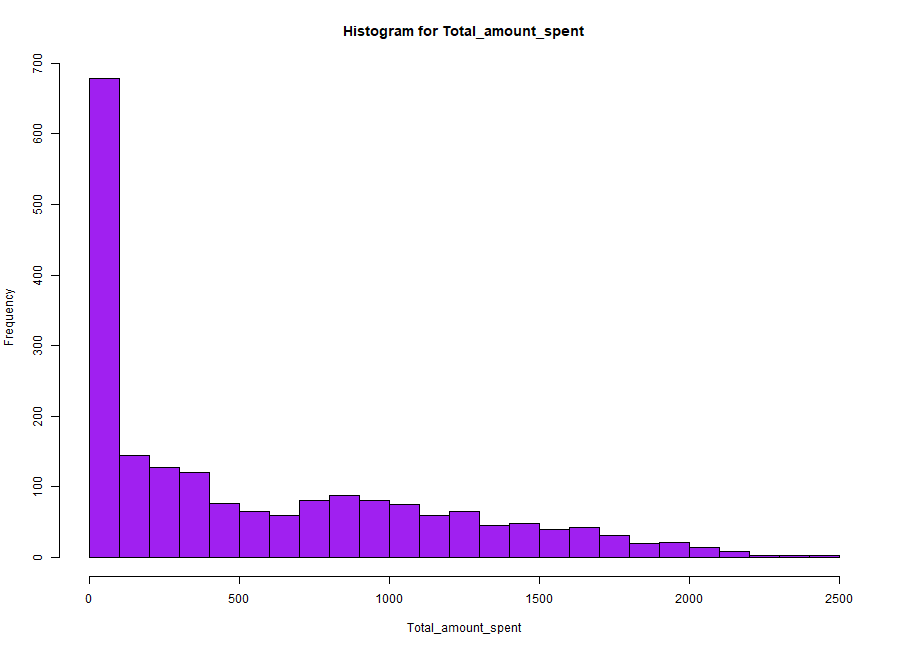
\includegraphics[width=\linewidth]{hist_Total_amount_spent.png}
  \caption{Total amount spent}
\end{subfigure}
\hfill
\begin{subfigure}{0.48\textwidth}
  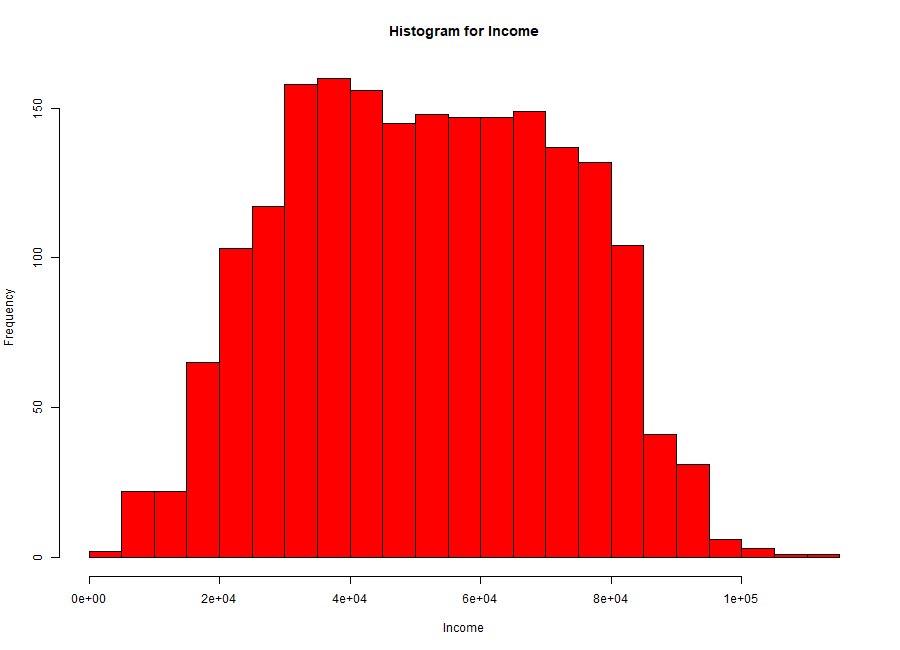
\includegraphics[width=\linewidth]{hist_Income.png}
  \caption{Income}
\end{subfigure}
\caption{Histograms of total spending (right-skewed) and income (roughly symmetric).}
\label{fig:uni}
\end{figure}

\paragraph{Outliers.} Using the $1.5 \times \text{IQR}$ rule, Income, Age, Recency, Customer\_Days and store purchases have no outliers. The spending columns have many (e.g.\ 220 for fruit, 166 for meat), but these come from the strong right skew rather than from errors: some customers simply spend much more than others. They are real customers, so all of them were kept.

\subsection{Categorical variables}
\begin{itemize}
  \item \textbf{Marital status:} married 777 (38.9\%), living together 505 (25.3\%), single 437, divorced 209 and widow 69 (3.5\%).
  \item \textbf{Education:} bachelor's 1,006 (50.4\%), master's 512, PhD 430 and high school only 49 (2.5\%).
  \item \textbf{Children:} 561 customers have no children, 1,017 have one, 374 have two and 45 have three.
  \item \textbf{Complaints:} only 19 customers (0.95\%) complained in the last 2 years.
\end{itemize}
Some groups (high school, widows, complainers, 3 children) are small, so tests involving them have low power.

\subsection{Normality}
A normality test only makes sense when the histogram looks roughly bell-shaped. From the histograms, 13 of the 15 variables are clearly not normal: spending and purchase counts are strongly right-skewed, and Recency and Customer\_Days are flat. These were not tested. Only Income and Age look roughly symmetric, so only these two were checked, with a normal Q-Q plot, the Kolmogorov--Smirnov (K-S) test and the Lilliefors test (Figure~\ref{fig:qq}).

\begin{itemize}
  \item \textbf{Income:} $D = 0.047$ (K-S $p = 0.0003$, Lilliefors $p < 0.001$).
  \item \textbf{Age:} $D = 0.058$ (K-S $p < 0.001$, Lilliefors $p < 0.001$).
\end{itemize}
Both tests reject normality for both variables. The Lilliefors test is the correct version here, because the mean and standard deviation are estimated from the same data, which makes the plain K-S test too lenient. The departures from normality are small ($D < 0.06$), but with about 2,000 customers even small differences are significant. The Q-Q plots show that the points bend away from the line at both ends: the distributions have a flatter top and thinner tails than a normal curve.

\textbf{Conclusion:} none of the numerical variables is normally distributed, so the rest of the analysis uses non-parametric methods (Spearman correlation, Wilcoxon and Kruskal--Wallis tests).

\begin{figure}[H]
\centering
\begin{subfigure}{0.48\textwidth}
  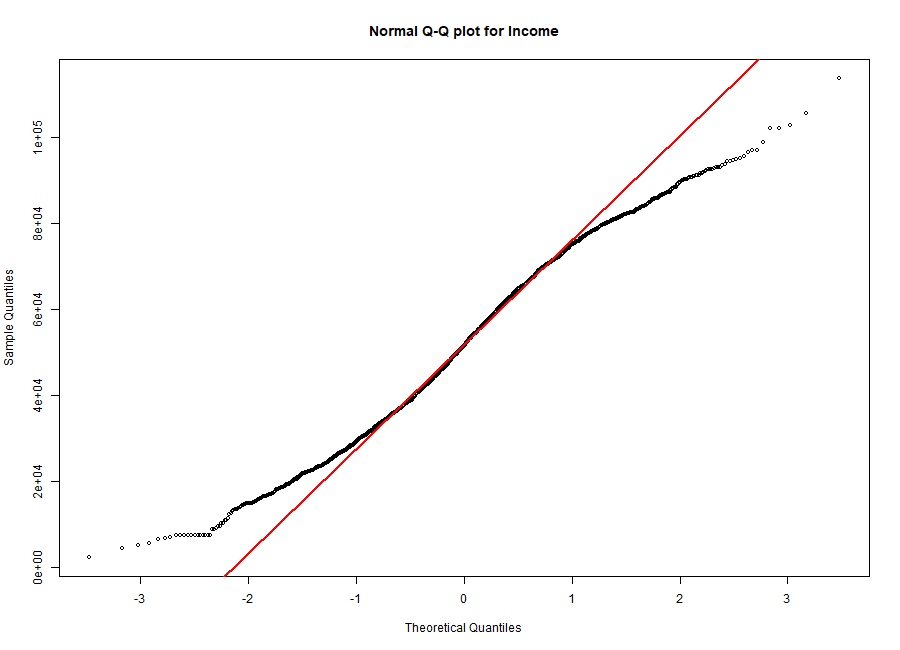
\includegraphics[width=\linewidth]{qq_Income.png}
  \caption{Income}
\end{subfigure}
\hfill
\begin{subfigure}{0.48\textwidth}
  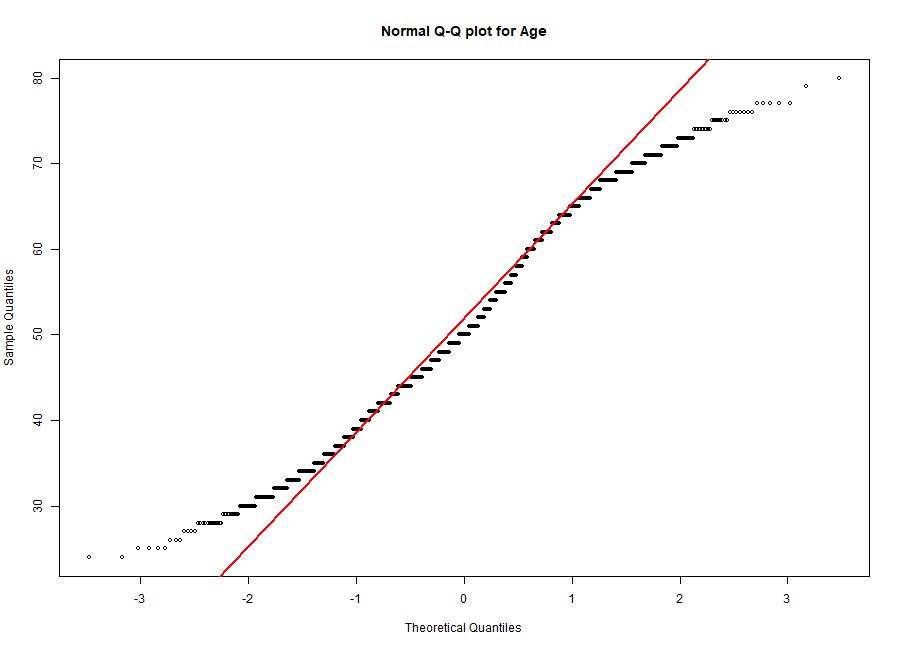
\includegraphics[width=\linewidth]{qq_Age.png}
  \caption{Age}
\end{subfigure}
\caption{Normal Q-Q plots of Income and Age.}
\label{fig:qq}
\end{figure}

% ==================================================================
\section{Bivariate Analysis}
% ==================================================================

\subsection{Correlations}
Figure~\ref{fig:heatmap} shows the Spearman correlations between the numerical variables. Spearman is used because the variables are skewed and it measures any monotonic (always increasing or always decreasing) relationship, not only a straight line.
\begin{itemize}
  \item Income has a very strong positive correlation with total spending ($\rho = 0.87$).
  \item Wine and meat spending each have $\rho = 0.94$ with total spending. This is mostly built in, since they are the two largest parts of the total.
  \item Website visits have a moderate negative correlation with spending ($\rho = -0.47$).
  \item Recency has almost no correlation with spending ($\rho = 0.02$).
\end{itemize}

\begin{figure}[H]
\centering
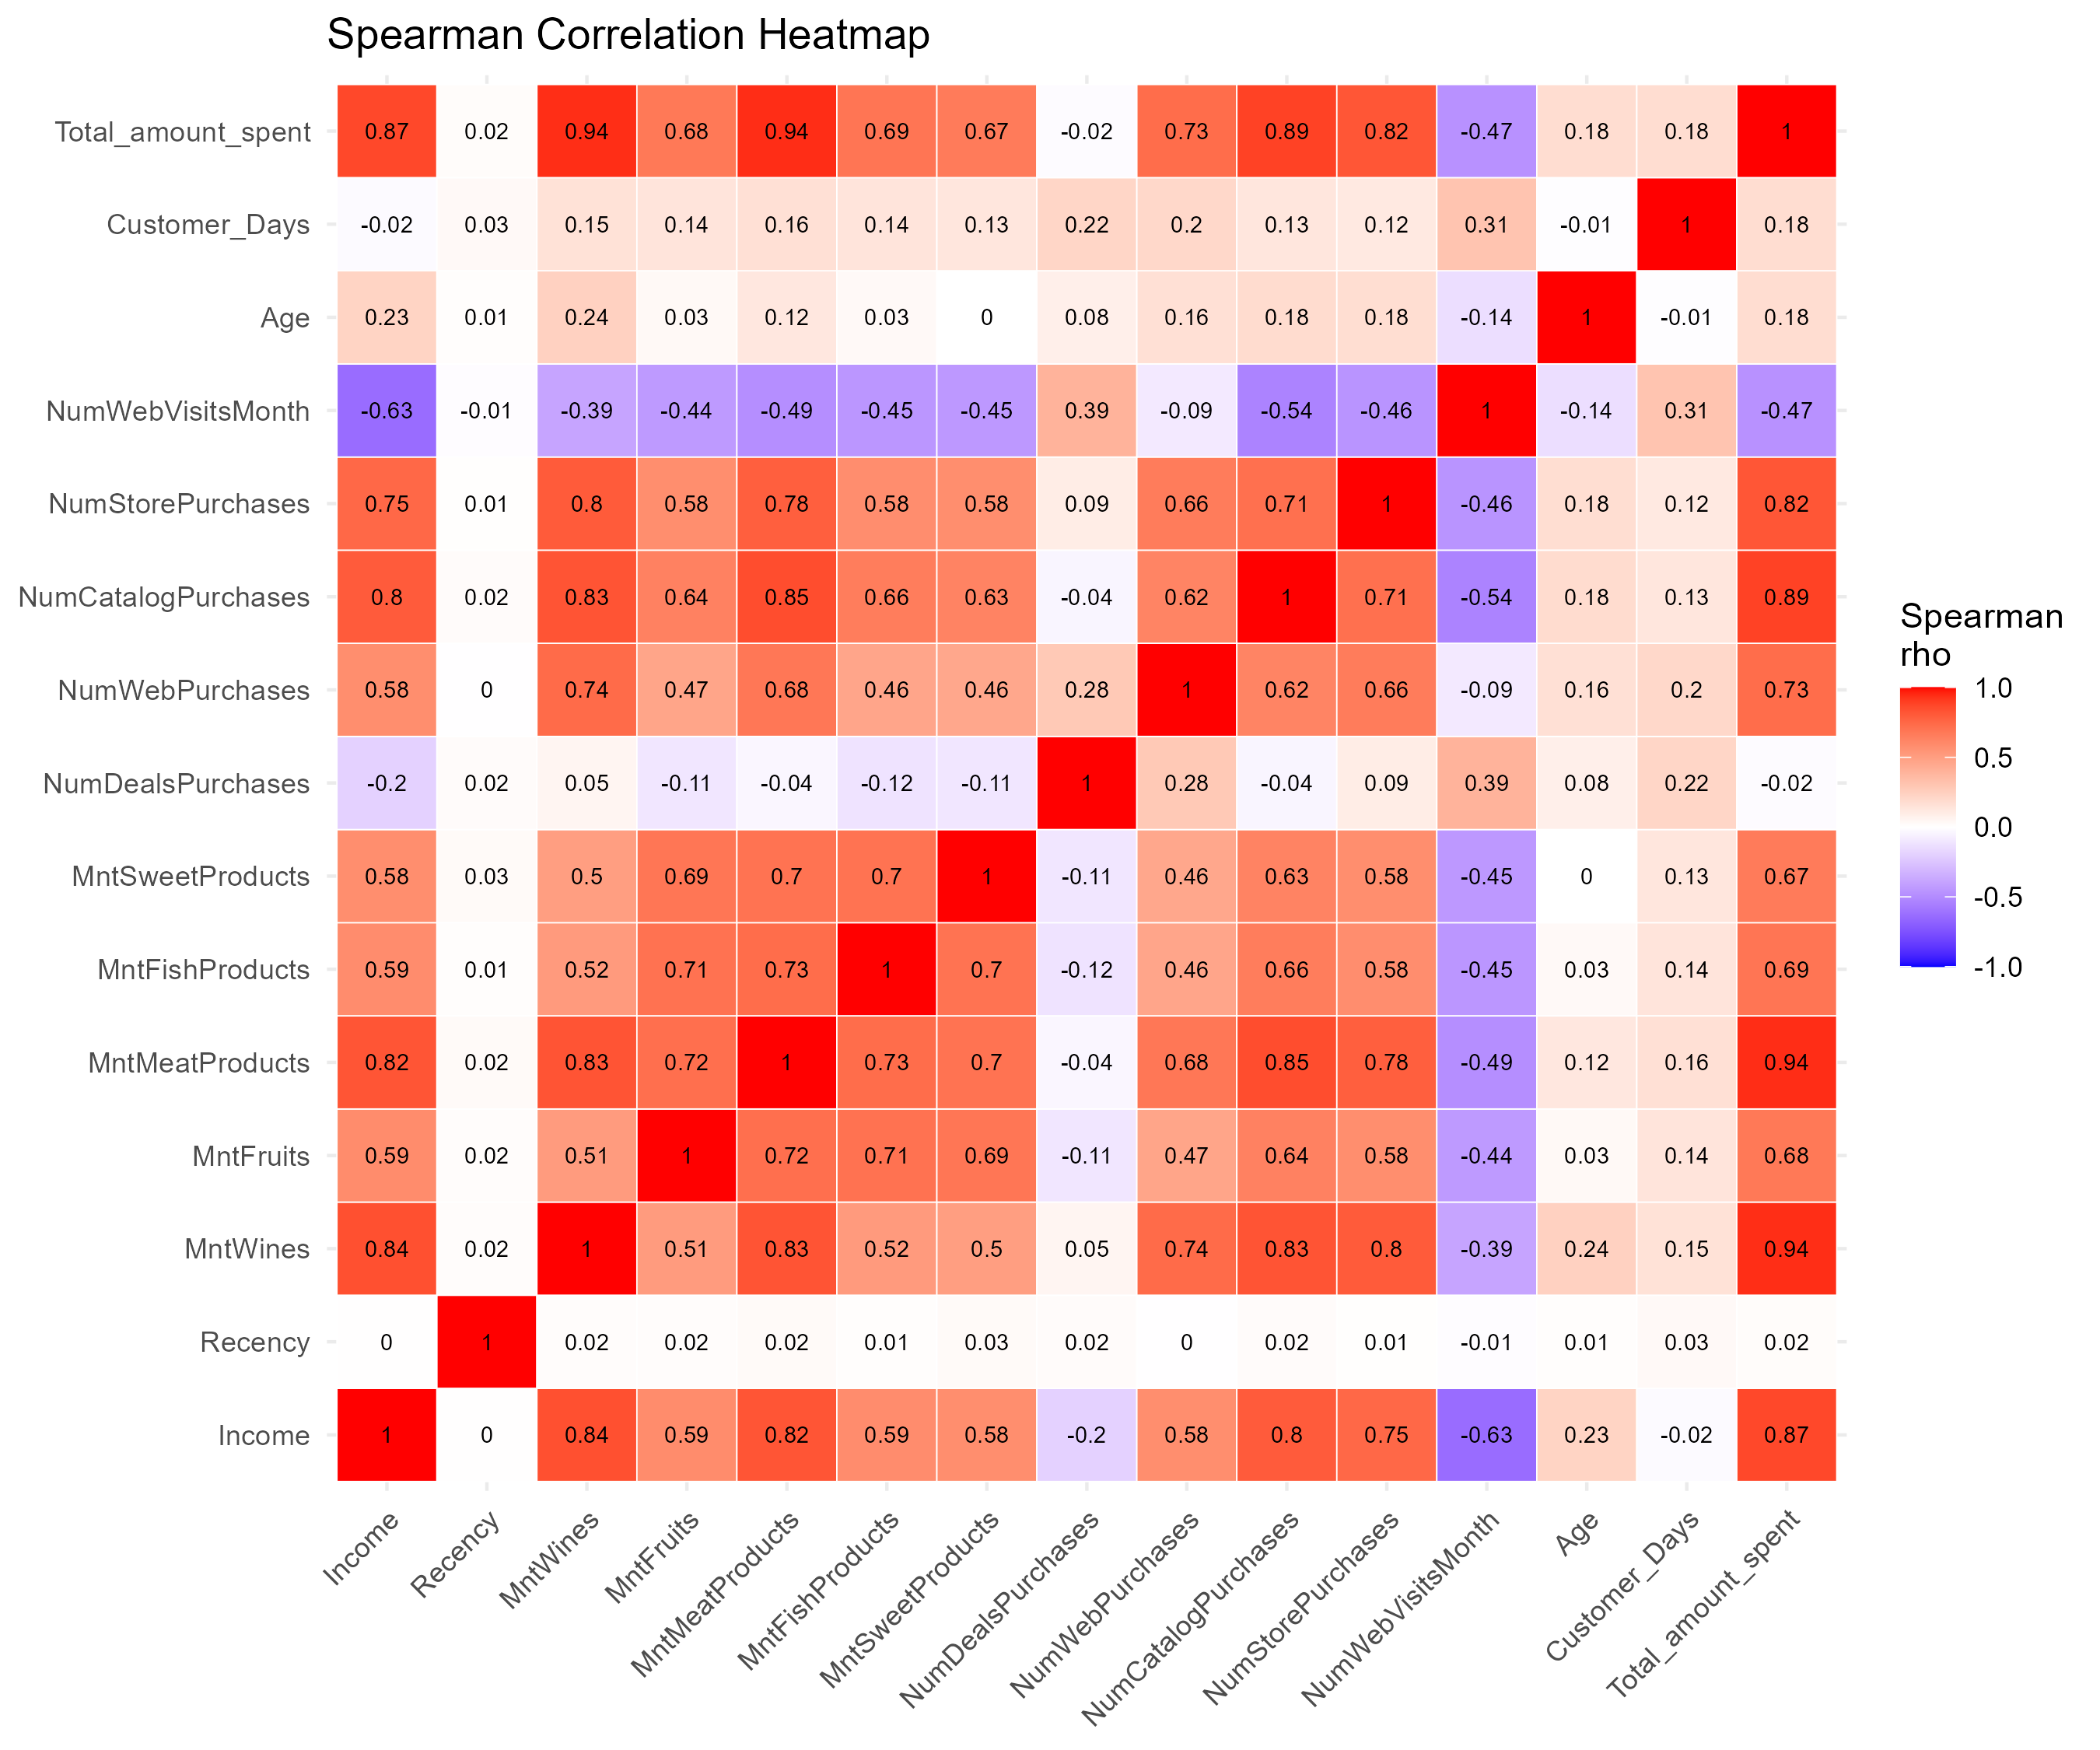
\includegraphics[width=0.75\textwidth]{heatmap_spearman.png}
\caption{Spearman correlation heatmap (red = positive, blue = negative).}
\label{fig:heatmap}
\end{figure}

\subsection{Income and spending}
Spending rises clearly with income, but not in a straight line (Figure~\ref{fig:income}): it stays low up to an income of about 40,000 and then rises steeply. Higher-income customers also buy more often: the average number of purchases rises from 5.5 in the lowest income quartile to 19.4 in the highest.

\begin{figure}[H]
\centering
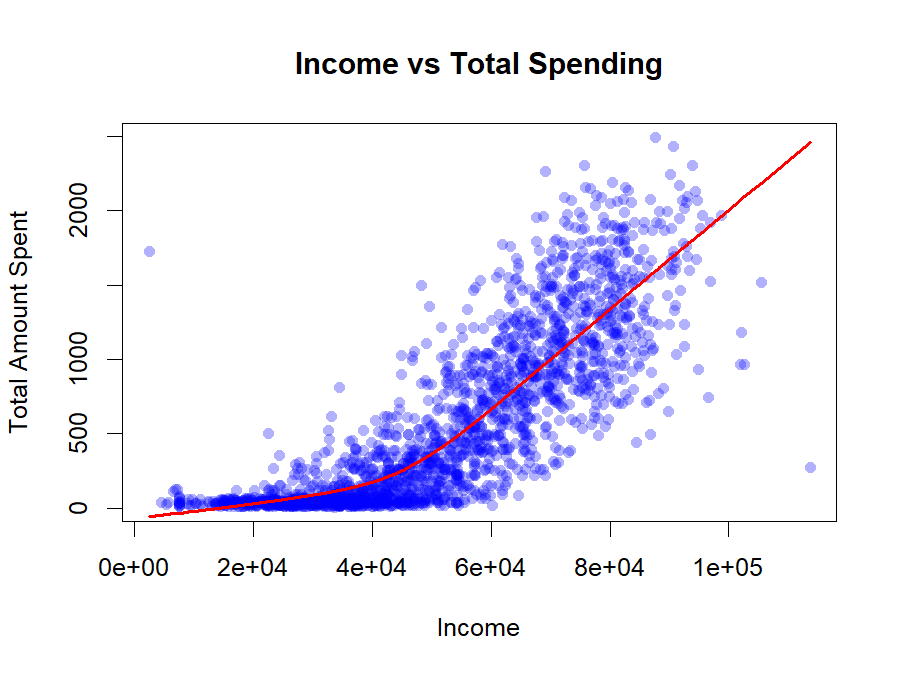
\includegraphics[width=0.7\textwidth]{scatter_income_spending.png}
\caption{Income vs total spending, with a smooth trend line (red).}
\label{fig:income}
\end{figure}

\subsection{Children, education and marital status}
\begin{itemize}
  \item \textbf{Children:} median spending falls with every extra child, from 1,117 with no children to 264 (1 child), 85 (2) and 62 (3) (Figure~\ref{fig:groups}a).
  \item \textbf{Education:} high-school customers spend much less (median 40) than the others. PhD customers have the highest median (448.5), but spending does not rise steadily with education: bachelor's (353) is above master's (297).
  \item \textbf{Marital status:} widows have the highest median spending (597), and the other groups are similar (303--350). The widow group is small (69) and older, so this may be an age effect (tested in Section~\ref{sec:tests}).
\end{itemize}

\begin{figure}[H]
\centering
\begin{subfigure}{0.48\textwidth}
  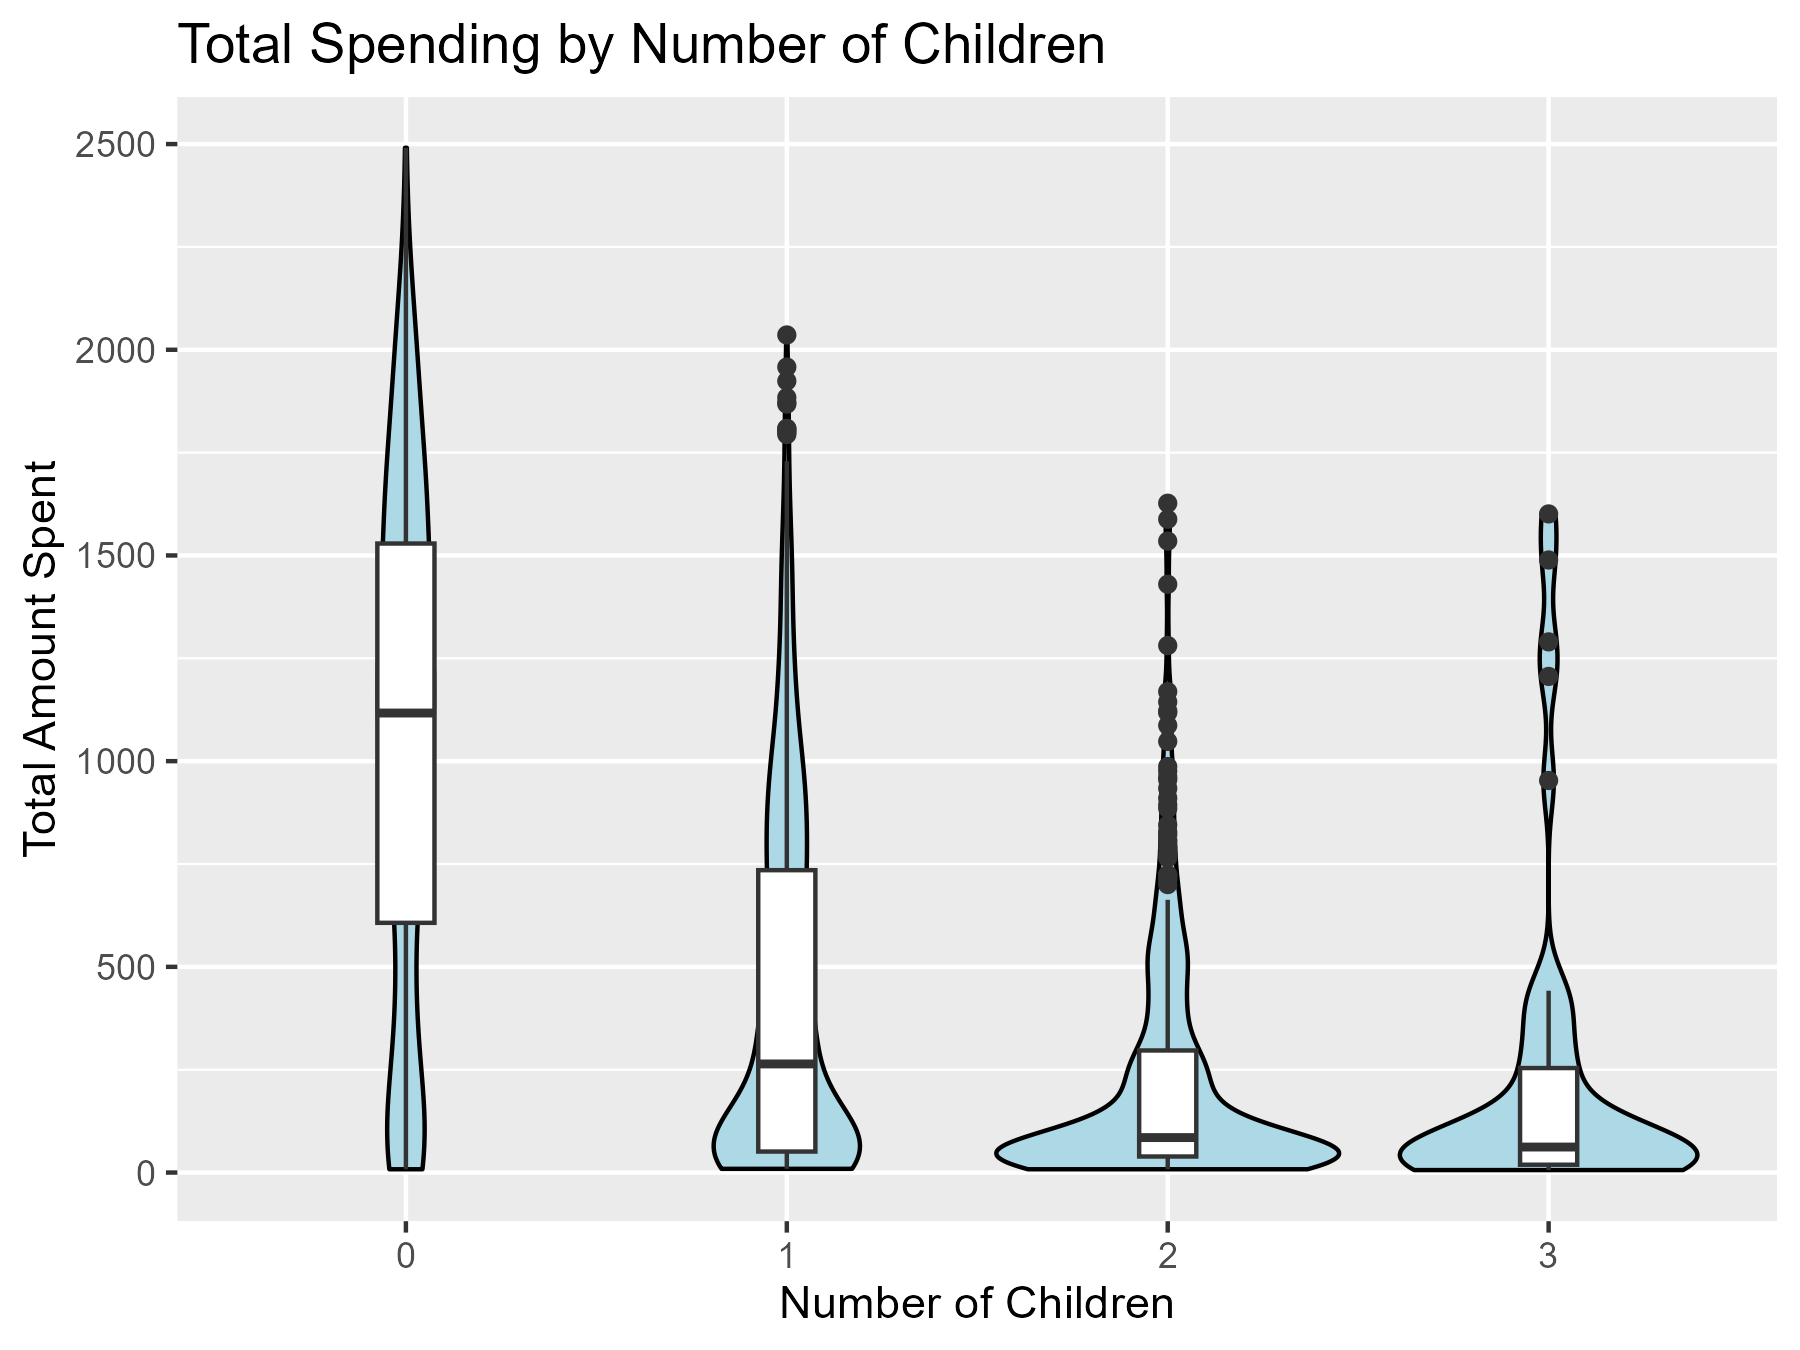
\includegraphics[width=\linewidth]{violin_spending_children.png}
  \caption{By number of children}
\end{subfigure}
\hfill
\begin{subfigure}{0.48\textwidth}
  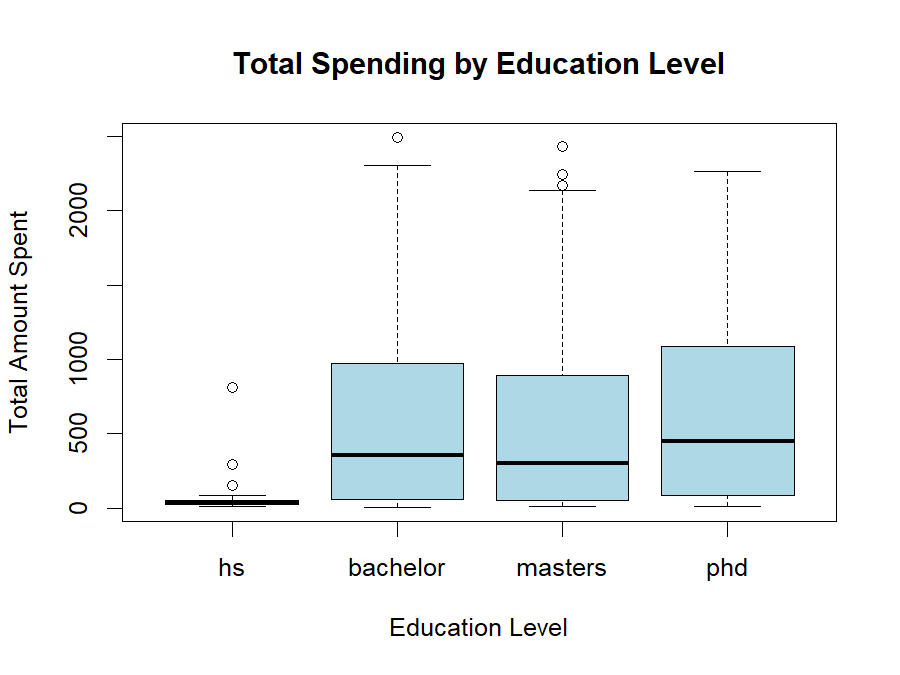
\includegraphics[width=\linewidth]{box_spending_education.png}
  \caption{By education level}
\end{subfigure}
\caption{Total spending by number of children and by education level.}
\label{fig:groups}
\end{figure}

\subsection{Purchase channels}
On average, half of a customer's purchases are made in store (50.5\%), a third on the website (33.2\%) and a sixth through the catalogue (16.4\%). The store is the main channel in every age group (Figure~\ref{fig:channels}).

\begin{figure}[H]
\centering
\begin{subfigure}{0.48\textwidth}
  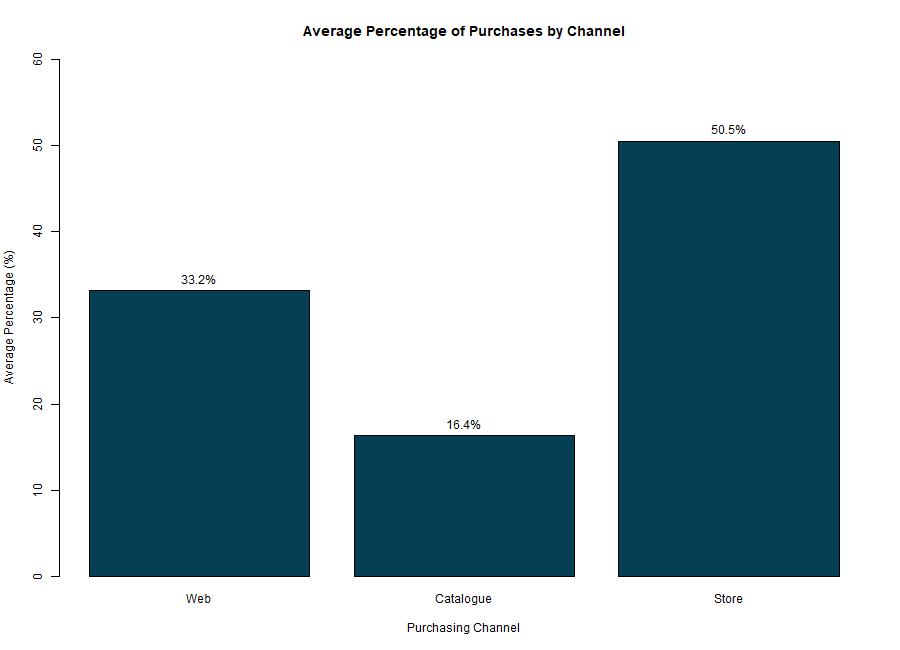
\includegraphics[width=\linewidth]{bar_channels.png}
  \caption{All customers}
\end{subfigure}
\hfill
\begin{subfigure}{0.48\textwidth}
  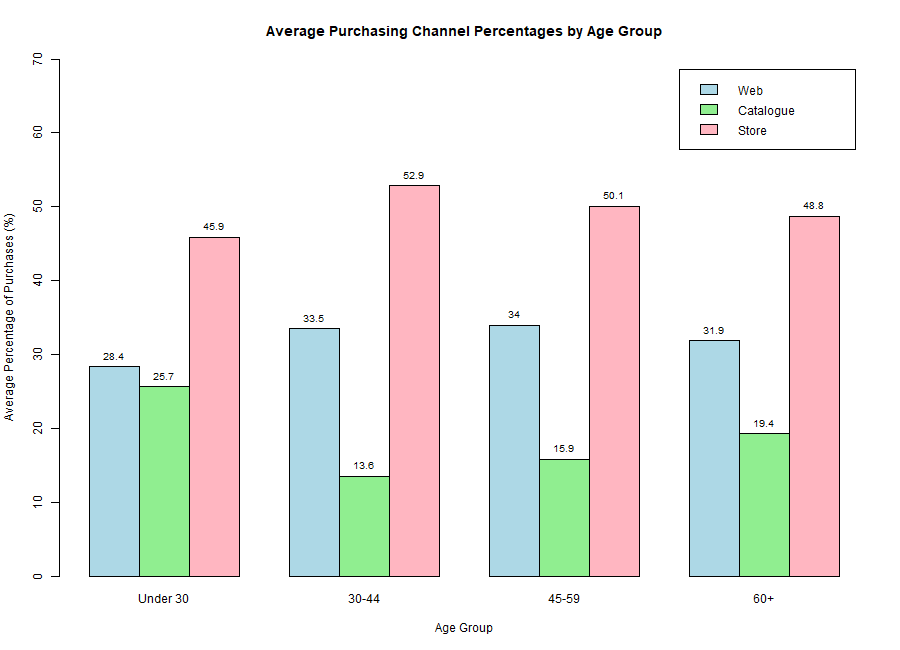
\includegraphics[width=\linewidth]{bar_channels_age.png}
  \caption{By age group}
\end{subfigure}
\caption{Average share of purchases made through each channel.}
\label{fig:channels}
\end{figure}

\subsection{Discounts}
Families and lower-income customers are clearly more price-sensitive (Figure~\ref{fig:deals}):
\begin{itemize}
  \item The average share of purchases made with a discount rises from 8.8\% for customers without children to 24.9\% with one child and about 43\% with two or three.
  \item It falls steadily with income: 36.4\% in the lowest quartile, 32.6\%, 19.7\% and only 7.6\% in the highest ($\rho = -0.73$).
\end{itemize}

\begin{figure}[H]
\centering
\begin{subfigure}{0.48\textwidth}
  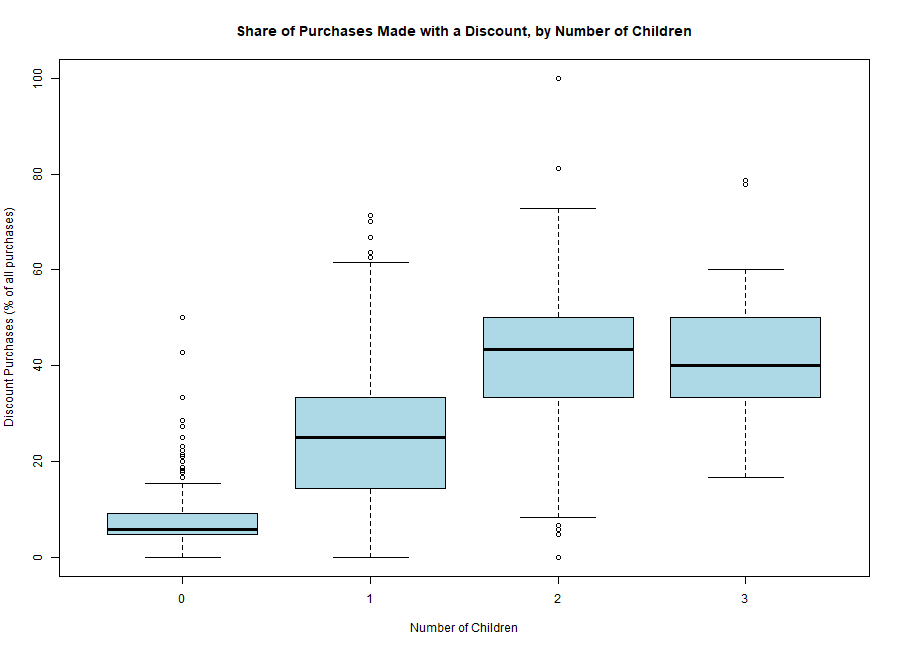
\includegraphics[width=\linewidth]{box_deals_children.png}
  \caption{By number of children}
\end{subfigure}
\hfill
\begin{subfigure}{0.48\textwidth}
  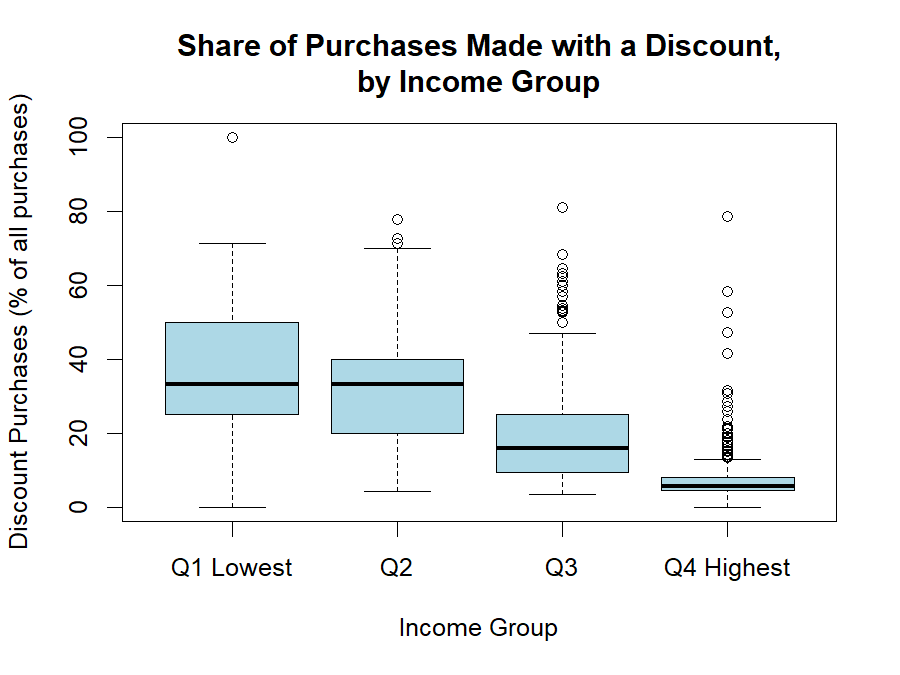
\includegraphics[width=\linewidth]{box_deals_income.png}
  \caption{By income group}
\end{subfigure}
\caption{Share of purchases made with a discount.}
\label{fig:deals}
\end{figure}

\subsection{Website visits}
Website visits do not turn into website purchases: the correlation is almost zero ($\rho = -0.09$), and customers make about 4 web purchases on average whatever their number of visits. The most frequent visitors are the lower-income, lower-spending customers: median income falls from \num{77382} (0--2 visits a month) to \num{31814} (9 or more), and median spending from 1,112 to 118. A possible explanation is that these customers browse the website for offers rather than to buy. Note that visits cover only the last month, while purchases cover a longer period.

\subsection{Recency and length of relationship}
How recently a customer last bought is not related to how much they spend ($\rho = 0.02$). The length of the relationship has a weak positive relationship with spending ($\rho = 0.18$): median spending rises from 150.5 for the newest quarter of customers to 523 for the longest-standing quarter. Spending covers the last 2 years only, and every customer has been with the company for at least 5.9 years, so all customers are compared over the same period.

% ==================================================================
\section{Hypothesis Testing}
\label{sec:tests}
% ==================================================================
Since no numerical variable is normal, we use non-parametric tests:
\begin{itemize}
  \item \textbf{Wilcoxon rank-sum test} to compare a numerical variable between two groups;
  \item \textbf{Kruskal--Wallis test} for three or more groups, followed by pairwise Wilcoxon tests (with the Benjamini--Hochberg correction) to find which groups differ;
  \item \textbf{Spearman correlation test} for two numerical variables;
  \item \textbf{Chi-square test of independence} for two categorical variables.
\end{itemize}
The significance level is 0.05. Table~\ref{tab:tests} summarises the results.

\begin{table}[H]
\centering
\small
\begin{tabular}{rllll}
\toprule
\# & Question & Test & Result & Decision \\
\midrule
1  & Spending: children vs no children & Wilcoxon & $p < 0.001$ & Reject $H_0$ \\
2  & Spending by number of children & Kruskal--Wallis & $p < 0.001$ & Reject $H_0$ \\
3  & Spending by education & Kruskal--Wallis & $p < 0.001$ & Reject $H_0$ \\
4  & Spending by marital status & Kruskal--Wallis & $p = 0.24$ & Do not reject \\
5  & Income vs spending & Spearman & $\rho = 0.87$, $p < 0.001$ & Reject $H_0$ \\
6  & Marital status vs education & Chi-square & $p = 0.26$ & Do not reject \\
7a & Income: complained vs not & Wilcoxon & $p = 0.22$ & Do not reject \\
7b & Spending: complained vs not & Wilcoxon & $p = 0.13$ & Do not reject \\
8  & Discount share by children & Kruskal--Wallis & $p < 0.001$ & Reject $H_0$ \\
9  & Discount share vs income & Spearman & $\rho = -0.73$, $p < 0.001$ & Reject $H_0$ \\
10 & Web visits vs web purchases & Spearman & $\rho = -0.09$, $p < 0.001$ & Reject $H_0$ \\
11 & Days as customer vs spending & Spearman & $\rho = 0.18$, $p < 0.001$ & Reject $H_0$ \\
12 & Recency vs spending & Spearman & $\rho = 0.02$, $p = 0.43$ & Do not reject \\
\bottomrule
\end{tabular}
\caption{Summary of the hypothesis tests. In each test, $H_0$ states that there is no difference between the groups (or no monotonic relationship).}
\label{tab:tests}
\end{table}

\paragraph{Children (tests 1, 2, 8).} Customers without children spend far more (median 1,117 vs 182). The pairwise tests show that spending falls with each extra child from 0 to 2, while the groups with 2 and 3 children do not differ significantly ($p = 0.15$). The discount share shows the same pattern in reverse: it rises from 0 to 2 children (medians 5.9\%, 25.0\% and 43.3\%, all pairs $p < 0.001$), and 2 and 3 children do not differ ($p = 0.9$).

\paragraph{Education (test 3).} High-school customers spend much less than every other level (all $p < 0.001$). PhD customers spend more than master's customers ($p = 0.004$), but bachelor's does not differ significantly from master's ($p = 0.10$) or PhD ($p = 0.07$). The clear finding is therefore high school versus the rest. The high-school group is small (49 customers).

\paragraph{Marital status (test 4).} There is no evidence that spending differs by marital status. Widows have the highest median, but they are also older (median age 63, vs 48--53 for the other groups), and older customers spend more ($\rho = 0.18$, $p < 0.001$). Among customers aged 60 and over, widows (median 606) spend about the same as non-widows (median 546; Wilcoxon $p = 0.67$). The higher spending of widows is therefore explained by their age, not by their marital status.

\paragraph{Complaints (test 7).} Customers who complained have lower medians (income \num{39684} vs \num{51566}; spending 89 vs 345), but the differences are not significant. With only 19 complainers, the tests have very little power, so we cannot conclude that there is no difference either.

\paragraph{Significant but weak (tests 10 and 11).} With about 2,000 customers, even very small correlations are statistically significant. The web visits correlation ($\rho = -0.09$) is significant but negligible in practice. A $p$-value tells us whether a relationship exists, while $\rho$ tells us how strong it is.

\paragraph{Multiple testing.} Running many tests at the 0.05 level increases the chance that some are significant by chance. After adjusting all $p$-values with the Benjamini--Hochberg correction, the conclusions do not change. Most significant $p$-values are below 0.001, so even the stricter Bonferroni threshold ($0.05/13 \approx 0.0038$) would give the same conclusions.

% ==================================================================
\section{Customer Segments and Regression}
% ==================================================================

\subsection{Principal Component Analysis}
Principal Component Analysis (PCA) summarises many variables with a few new axes, called principal components, that keep as much of the variation as possible. We applied it to 10 variables describing customer behaviour: income, the five spending columns, the three purchase channels and website visits. The variables were standardised first, so that income does not dominate.

The first component (PC1) explains 56\% of the variation and the second (PC2) another 12\%, so together they keep 68\% of the information in the 10 variables (Table~\ref{tab:pca}).
\begin{itemize}
  \item \textbf{PC1: overall buying power.} Income, all the spending columns and all the purchase channels have similar loadings, and website visits has the opposite sign. The sign of a component is arbitrary. Here a \emph{low} PC1 score means high income and high spending.
  \item \textbf{PC2: online wine buyers.} It is highest for web purchases, web visits and wine, and negative for fish, fruit and sweets.
\end{itemize}
Most of the differences between customers therefore come down to one thing: how much they earn and spend. The second, much smaller difference is whether they buy online and buy wine, or buy more fresh and sweet products.

\begin{table}[H]
\centering
\small
\begin{tabular}{lrr}
\toprule
Variable & PC1 & PC2 \\
\midrule
Income              & $-0.38$ & 0.07 \\
MntWines            & $-0.32$ & 0.40 \\
MntFruits           & $-0.30$ & $-0.24$ \\
MntMeatProducts     & $-0.35$ & $-0.14$ \\
MntFishProducts     & $-0.31$ & $-0.26$ \\
MntSweetProducts    & $-0.30$ & $-0.21$ \\
NumWebPurchases     & $-0.23$ & 0.63 \\
NumCatalogPurchases & $-0.35$ & 0.01 \\
NumStorePurchases   & $-0.32$ & 0.24 \\
NumWebVisitsMonth   & 0.27    & 0.44 \\
\midrule
Variance explained  & 56\% & 12\% \\
\bottomrule
\end{tabular}
\caption{Loadings of the first two principal components.}
\label{tab:pca}
\end{table}

\subsection{Clustering with k-means}
To find groups of customers with similar behaviour, we used k-means clustering on the same 10 variables: income, the five spending columns, the three purchase channels and website visits. Total spending was left out because it is the sum of the spending columns. All variables were standardised first (mean 0, SD 1), so that income, measured in tens of thousands, does not dominate the purchase counts.

\paragraph{Choosing the number of clusters.} Two methods were used (Figure~\ref{fig:k}):
\begin{itemize}
  \item \textbf{Elbow method:} the within-cluster sum of squares drops sharply from $k = 1$ to 2 and from 2 to 3, and then flattens, so the elbow is at $k = 2$--3.
  \item \textbf{Silhouette method:} the average silhouette width is highest for $k = 2$ (0.43), followed by $k = 3$ (0.35).
\end{itemize}
We chose $k = 3$. With $k = 2$ the customers are only split into high and low spenders, while $k = 3$ also separates a distinct middle group, which is more useful for describing customer profiles. Its silhouette (0.35) is still reasonable, and it sits at the elbow.

\begin{figure}[H]
\centering
\begin{subfigure}{0.48\textwidth}
  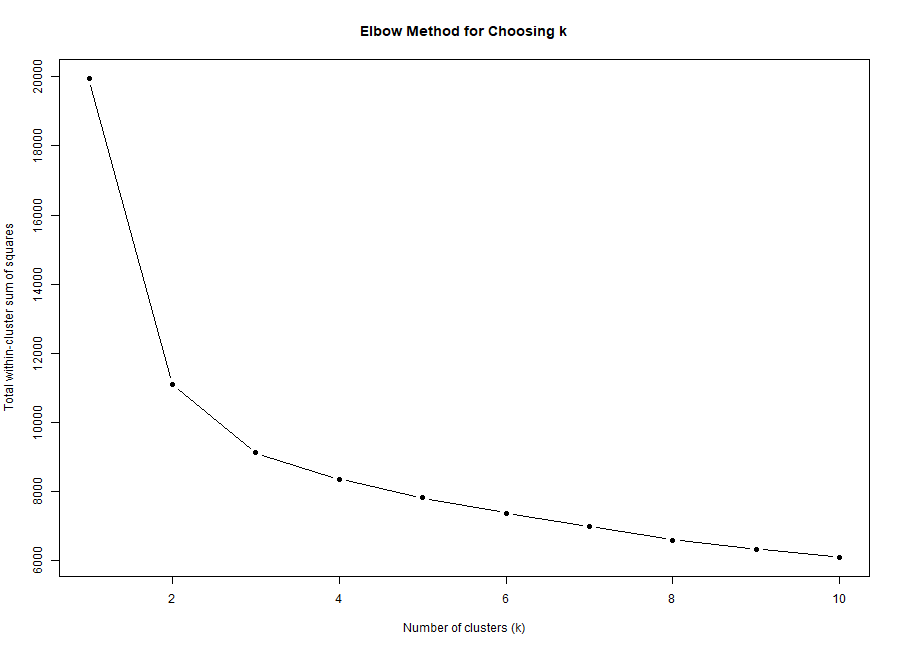
\includegraphics[width=\linewidth]{cluster_elbow.png}
  \caption{Elbow method}
\end{subfigure}
\hfill
\begin{subfigure}{0.48\textwidth}
  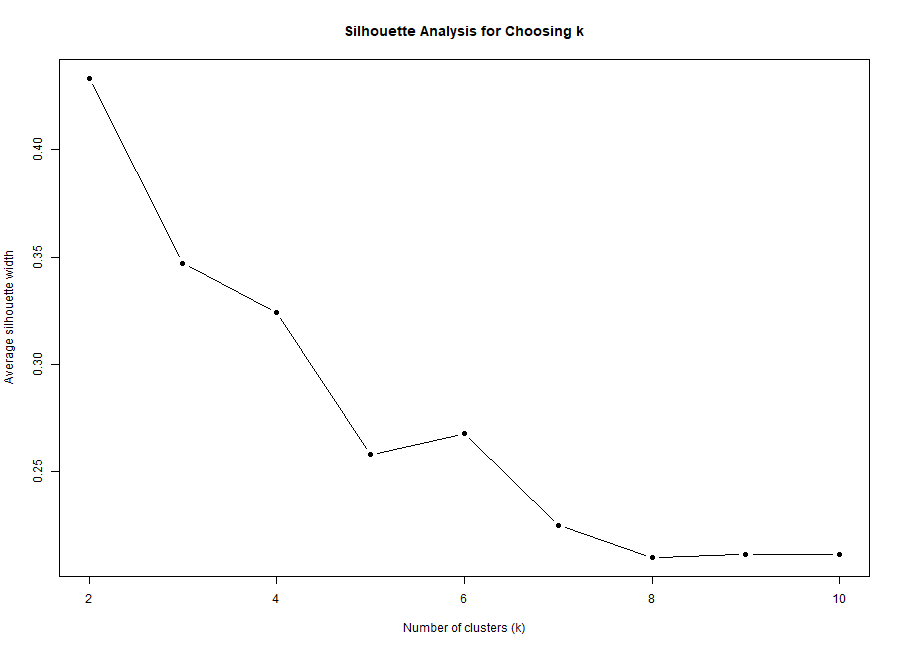
\includegraphics[width=\linewidth]{cluster_silhouette.png}
  \caption{Silhouette method}
\end{subfigure}
\caption{Choosing the number of clusters.}
\label{fig:k}
\end{figure}

\paragraph{The three segments.} Table~\ref{tab:clusters} describes each cluster using the medians of the original variables. Age, children and the purchase shares were not used to build the clusters, but they help describe them.

\begin{table}[H]
\centering
\small
\begin{tabular}{lrrr}
\toprule
 & \textbf{1. Budget} & \textbf{2. Affluent} & \textbf{3. Established} \\
 & \textbf{families} & \textbf{big spenders} & \textbf{families} \\
\midrule
Customers            & 960      & 491      & 546 \\
Income               & \num{35081} & \num{76412} & \num{59987} \\
Total spending       & 54       & 1,290    & 652 \\
Wine spending        & 23       & 548      & 434 \\
Meat spending        & 15       & 435      & 127 \\
Age                  & 48       & 51       & 54 \\
Have children        & 89\%     & 25\%     & 84\% \\
Discount share       & 33\%     & 6\%      & 15\% \\
Web share            & 33\%     & 26\%     & 36\% \\
Catalogue share      & 0\%      & 30\%     & 16\% \\
Store share          & 57\%     & 43\%     & 46\% \\
Web visits per month & 7        & 2        & 6 \\
\bottomrule
\end{tabular}
\caption{Cluster profiles (medians, except ``Have children'').}
\label{tab:clusters}
\end{table}

\begin{itemize}
  \item \textbf{Budget families} (960 customers, the largest group): the lowest income and very low spending. Almost all have children. A third of their purchases are made with a discount, mostly in store, and they almost never use the catalogue. They visit the website often but buy little there.
  \item \textbf{Affluent big spenders} (491): the highest income and spending, especially on wine and meat. Most have no children. They rarely use discounts and use the catalogue the most.
  \item \textbf{Established families} (546): mid-to-high income and spending, mostly on wine. Most have children, and they are slightly older. They use some discounts and buy online the most.
\end{itemize}

Figure~\ref{fig:clusters} shows that budget families are clearly separated from the other two groups by income and spending. Clusters 2 and 3 overlap at mid-to-high incomes: they differ less in income and more in \emph{how} they buy (children, catalogue vs web, wine vs meat), which a two-variable plot cannot show. Five of the ten clustering variables are spending columns, so spending has a large weight in the clustering, which is why the clusters follow spending level closely.

The PCA plot separates the clusters much better (Figure~\ref{fig:pca}). Along PC1 they are ordered by buying power: affluent big spenders (median PC1 score $-3.27$), established families ($-0.59$) and budget families ($2.20$). Along PC2, established families score highest (median 1.06), because they buy online and buy wine the most. So clusters 2 and 3, which overlap in income, are told apart by \emph{how} they buy.

\begin{figure}[H]
\centering
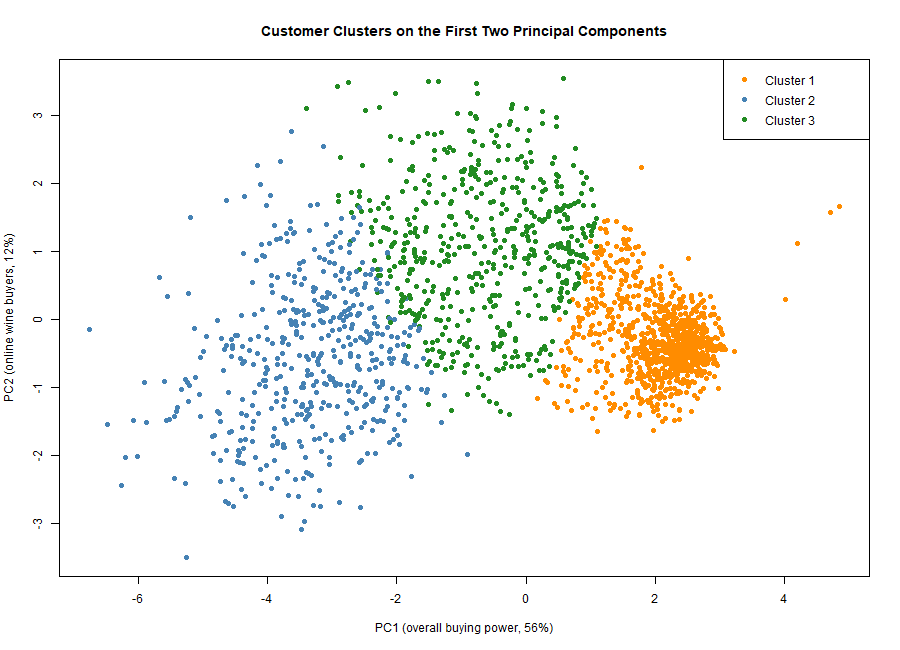
\includegraphics[width=0.75\textwidth]{cluster_pca.png}
\caption{Customers on the first two principal components, coloured by cluster.}
\label{fig:pca}
\end{figure}

\begin{figure}[H]
\centering
\begin{subfigure}{0.48\textwidth}
  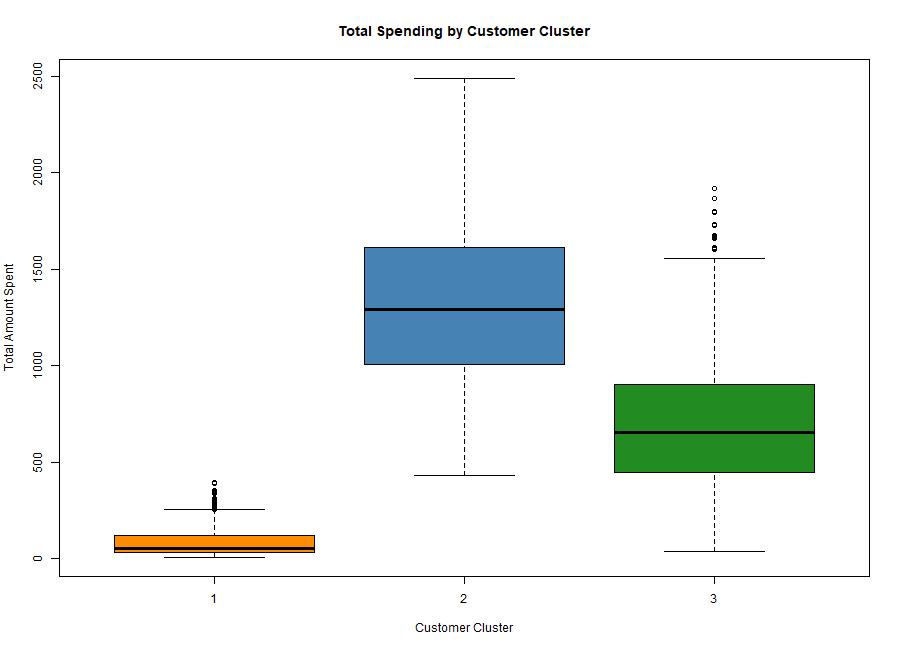
\includegraphics[width=\linewidth]{cluster_spending_boxplot.png}
  \caption{Total spending by cluster}
\end{subfigure}
\hfill
\begin{subfigure}{0.48\textwidth}
  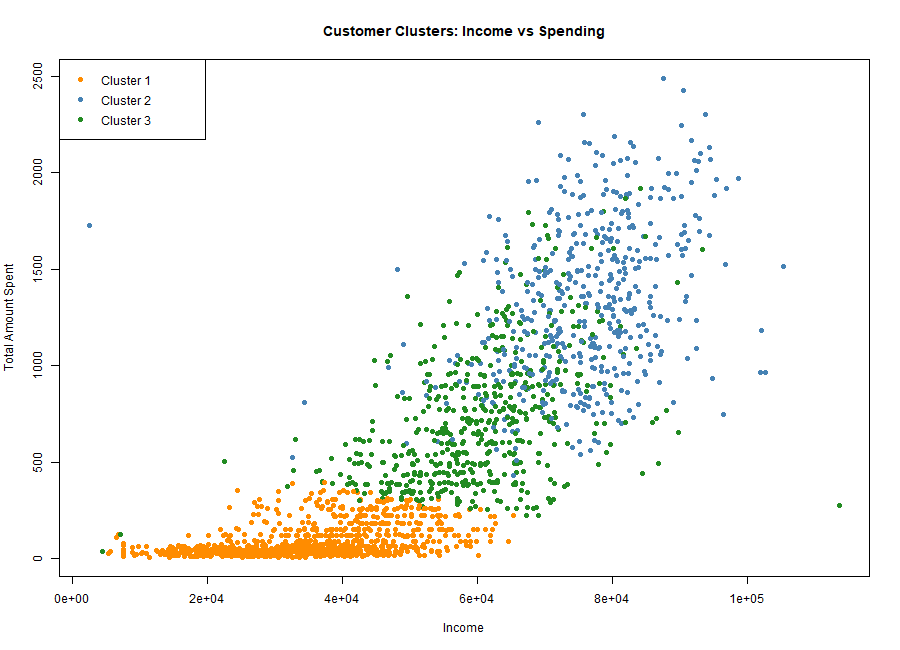
\includegraphics[width=\linewidth]{cluster_income_vs_spending.png}
  \caption{Income vs spending, coloured by cluster}
\end{subfigure}
\caption{The three customer segments.}
\label{fig:clusters}
\end{figure}

\subsection{Regression: what explains spending?}
The tests in Section~\ref{sec:tests} look at one variable at a time. Income, children, age and education are related to each other, so we fitted a linear regression to measure the effect of each one \emph{while holding the others fixed}. Spending is strongly right-skewed, so the response is $\log(\text{Total\_amount\_spent})$, which is much more symmetric (the minimum spending is 6, so there are no zeros):
\[
\log(\text{Spending}) = \beta_0 + \beta_1\,\text{Income} + \beta_2\,\text{Children} + \beta_3\,\text{Age} + \text{Education} + \text{Marital status} + \varepsilon .
\]
With a log response, a coefficient $\beta$ means that spending changes by about $(e^{\beta} - 1) \times 100\%$ for a one-unit increase in that predictor. High school and divorced are the reference groups.

\begin{table}[H]
\centering
\small
\begin{tabular}{lrrl}
\toprule
Predictor & Coefficient & $p$-value & Effect on spending \\
\midrule
Income (per \num{10000}) & 0.577 & $< 0.001$ & $+78\%$ \\
Children (per child)    & $-0.344$ & $< 0.001$ & $-29\%$ \\
Age (per year)          & 0.0045 & 0.006 & $+0.45\%$ \\
Education (vs high school) & 0.01 to 0.05 & all $> 0.6$ & not significant \\
Marital status (vs divorced) & $-0.01$ to 0.08 & all $> 0.4$ & not significant \\
\bottomrule
\end{tabular}
\caption{Regression of $\log(\text{spending})$. $R^2 = 0.73$.}
\label{tab:reg}
\end{table}

\begin{itemize}
  \item \textbf{Income} is the strongest predictor: \num{10000} more income goes with about 78\% higher spending.
  \item \textbf{Each extra child} goes with about 29\% lower spending \emph{at the same income}. Children therefore reduce spending on their own, not only because families with children earn less.
  \item \textbf{Age} has a small positive effect (about 0.45\% per year).
  \item \textbf{Education is not significant} once income is in the model. The low spending of high-school customers (test 3) is therefore mostly explained by their lower income.
  \item \textbf{Marital status is not significant}, which agrees with test 4.
  \item The model explains 73\% of the variation in log(spending) ($R^2 = 0.73$), mostly through income and children.
\end{itemize}

\paragraph{Model checks.} Figure~\ref{fig:diag} shows the diagnostic plots. The residuals are roughly normal (the Q-Q plot follows the line except for a few extreme customers), and no customer has a large influence on the model. However, the residuals-vs-fitted plot shows a curve rather than a flat line, and the spread of the residuals is a little uneven. This means the model does not fully capture the curved effect of income seen in Figure~\ref{fig:income}: spending stays low and then rises steeply. The model fits well overall, but this is a limitation.

\begin{figure}[H]
\centering
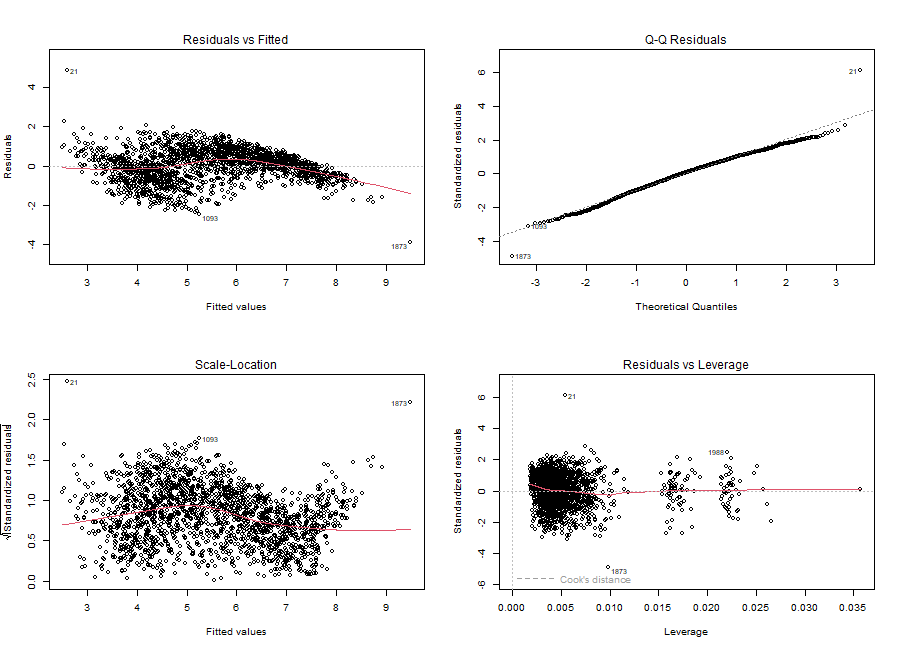
\includegraphics[width=0.8\textwidth]{regression_diagnostics.png}
\caption{Diagnostic plots of the regression model.}
\label{fig:diag}
\end{figure}

% ==================================================================
\section{Conclusions and Recommendations}
% ==================================================================
\subsection{Main findings}
\begin{enumerate}
  \item \textbf{Income is the main driver of spending} ($\rho = 0.87$; +78\% spending per \num{10000} of income).
  \item \textbf{Children reduce spending strongly}, even at the same income (about $-29\%$ per child), and families rely much more on discounts.
  \item \textbf{Lower-income customers are more price-sensitive}: their share of discounted purchases is much higher ($\rho = -0.73$).
  \item \textbf{Education and marital status matter little.} High-school customers spend less, but this is explained by their income. The higher spending of widows is explained by their age.
  \item \textbf{Website visits do not turn into website purchases.} The most frequent visitors are low-income, low-spending customers.
  \item \textbf{The store is the main channel} (about half of all purchases) in every age group.
  \item \textbf{There are three customer segments}: budget families, affluent big spenders and established families.
\end{enumerate}

\subsection{Recommendations for the company}
\begin{itemize}
  \item \textbf{Budget families:} target them with discounts and family offers, mainly in store. Since they visit the website often but rarely buy there, online offers could help turn their visits into purchases.
  \item \textbf{Affluent big spenders:} focus on premium wine and meat products, through the catalogue. Discounts are not needed to keep them.
  \item \textbf{Established families:} this group buys online the most and spends a lot on wine, so it is a good target for online wine promotions.
  \item \textbf{Website:} investigate why visits do not lead to purchases, for example the checkout process or the offers shown to frequent visitors.
\end{itemize}

% ==================================================================
\section{Limitations}
% ==================================================================
\begin{itemize}
  \item \textbf{Small groups:} high school (49), widows (69), 3 children (45) and complainers (19). Tests on these groups have low power.
  \item \textbf{Different time periods:} website visits cover only the last month, while spending and purchases cover the last 2 years.
  \item \textbf{Correlation is not causation:} the analysis shows associations, not causes. For example, children are related to lower spending, but other factors linked to having children may also play a role.
  \item \textbf{Regression:} the straight-line model does not fully capture the curved effect of income.
  \item \textbf{Clustering:} the choice of $k = 3$ is partly a judgement call ($k = 2$ had a higher silhouette), and the result depends on which variables are used.
  \item \textbf{Duplicates:} we assumed that the 203 identical rows are repeated entries. If some were real customers, a small amount of data was lost.
\end{itemize}

% ==================================================================
\appendix
\section{R Code}
% ==================================================================
The analysis is submitted as a commented R file. It is organised in the following parts:
\begin{enumerate}
  \item Setup: file paths, the function that saves figures and the lists of column names.
  \item Cleaning: import, logic checks, cleaning and new variables.
  \item Descriptive analysis: summary statistics, outliers, categorical variables and normality.
  \item Bivariate analysis: correlations, group comparisons and scatterplots.
  \item Hypothesis tests.
  \item PCA, clustering and regression.
\end{enumerate}
The R packages used are \texttt{e1071} (skewness and kurtosis), \texttt{nortest} (Lilliefors test), \texttt{ggplot2} (violin plot) and \texttt{cluster} (silhouette).

\end{document}
